\documentclass[11pt]{article}
\usepackage[margin=1in]{geometry}
\usepackage{amsmath, amssymb}
\usepackage{enumitem}
\usepackage{tikz}
\usepackage{tikz-qtree}
\usetikzlibrary{arrows.meta, positioning, graphs, automata, matrix, calc}

\setlength{\parindent}{0pt}
\setlength{\parskip}{0.5em}
\setlist{nosep}

\tikzset{
    every tree node/.style={circle, draw, minimum size=0.6cm, inner sep=1pt},
    blank/.style={draw=none, fill=none, edge from parent/.style={draw=none}},
    blacknode/.style={circle, draw, fill=black, text=white, minimum size=0.6cm, inner sep=1pt},
    whitenode/.style={circle, draw, fill=white, text=black, minimum size=0.6cm, inner sep=1pt},
    rednode/.style={circle, draw, fill=white, text=black, minimum size=0.6cm, inner sep=1pt},
    tfnode/.style={rectangle, draw, rounded corners=2pt, minimum size=0.45cm, inner sep=1pt},
    listnode/.style={rectangle, draw, rounded corners=2pt, minimum height=0.6cm, inner sep=3pt},
    skipnode/.style={rectangle, draw, minimum size=0.6cm, inner sep=2pt},
    main node/.style={circle, draw, minimum size=0.6cm}
}
\begin{document}

\begin{center}
    \Large\textbf{CS 253: Data Structures and Algorithms}\\
    \large\textbf{Randomized Final Study Problem}
\end{center}
\vspace{1em}

% seed=1
% topic=skip_list
% promotions=6
% max_height=5

\section*{Sequence-Based Structures}
\subsection*{Skip List Tracing Challenge}
Construct a skip list by inserting the keys in \texttt{[66, 36, 56, 58, 90, 27, 51, 75, 94, 91]}. Use the prescribed tower heights in the table below to remove coin-flip ambiguity. After the structure is built, remove the keys in \texttt{[36, 75, 91]}, showing each pointer update.

\begin{center}
\begin{tabular}{|c|c|c|c|c|c|c|c|c|c|c|}
\hline
 Key & 66 & 36 & 56 & 58 & 90 & 27 & 51 & 75 & 94 & 91 \\
\hline
 Height & 1 & 1 & 5 & 1 & 1 & 1 & 3 & 1 & 1 & 1 \\
\hline
\end{tabular}
\end{center}

\subsection*{Instructor Reference}
Promotions above the base level: 6. Final skip list after the deletions:
\begin{center}
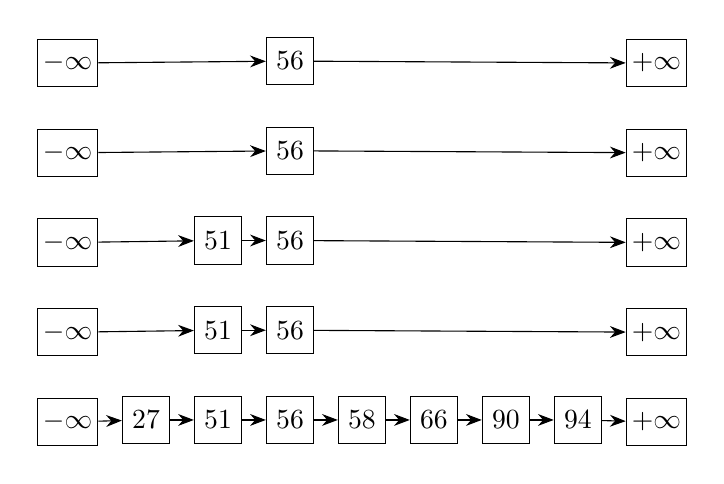
\begin{tikzpicture}[>={Stealth[length=2mm]}]
\matrix (m) [matrix of nodes, nodes={skipnode}, column sep=0.3cm, row sep=0.5cm] {
    $-\infty$ &  &  & 56 &  &  &  &  & $+\infty$ \\
    $-\infty$ &  &  & 56 &  &  &  &  & $+\infty$ \\
    $-\infty$ &  & 51 & 56 &  &  &  &  & $+\infty$ \\
    $-\infty$ &  & 51 & 56 &  &  &  &  & $+\infty$ \\
    $-\infty$ & 27 & 51 & 56 & 58 & 66 & 90 & 94 & $+\infty$ \\
};
\draw[->] (m-1-1) -- (m-1-4);
\draw[->] (m-1-4) -- (m-1-9);
\draw[->] (m-2-1) -- (m-2-4);
\draw[->] (m-2-4) -- (m-2-9);
\draw[->] (m-3-1) -- (m-3-3);
\draw[->] (m-3-3) -- (m-3-4);
\draw[->] (m-3-4) -- (m-3-9);
\draw[->] (m-4-1) -- (m-4-3);
\draw[->] (m-4-3) -- (m-4-4);
\draw[->] (m-4-4) -- (m-4-9);
\draw[->] (m-5-1) -- (m-5-2);
\draw[->] (m-5-2) -- (m-5-3);
\draw[->] (m-5-3) -- (m-5-4);
\draw[->] (m-5-4) -- (m-5-5);
\draw[->] (m-5-5) -- (m-5-6);
\draw[->] (m-5-6) -- (m-5-7);
\draw[->] (m-5-7) -- (m-5-8);
\draw[->] (m-5-8) -- (m-5-9);
\end{tikzpicture}
\end{center}

\end{document}
